\lez{25}{20-04-2020}{}
\subsection{Approssimazione di onda rotante}%
\label{sub:Approssimazione di onda rotante}
Ricordiamo la forma della perturbazione con una onda monocromatica incidente:
\[
    \hat{V}(t) = W^+ e^{-i\omega t}+W^-e^{i\omega t}
.\] 
La prima parte descrive i processi di assorbimento, l'altra i processi di emissione stimolata.\\
Prendendo il sistema a due livelli introdotto a fine della scorsa lezione abbiamo visto che il primo termine della perturbazione inserito nella regola d'oro di fermi porta un contributo del tipo  $\delta (E_1-E_2-\hbar \omega) $. Questo termine è diverso da zero quando $\hbar \omega = E_1 -E_2$.\\
L'altro termine invece produce $\delta (E_f-E_1 + \hbar \omega)$ quindi questo descrive un processo in cui l'energia dello stato finale è minore di quella dello stato iniziale.\\
Se fossimo in una situazione in cui la regola d'oro non è invece applicabile abbiamo che le funzioni avranno un certo allargamento con code oscillanti (le funzioni $F$ della scorsa lezione). 
\begin{defn}[Approssimazione di onda rotante]{defn:Approssimazione di onda rotante}
L'approssimazione di onda rotante (RWA) consiste nel trascurare nei processi di assorbimento il termine con il $W^-$ e nei processi di emissione il termine con il $W^+$.
\end{defn}
In pratica tale approssimazione funziona bene quando i due picchi delle funzioni per $W^+$ e $W^-$ sono lontani:
\begin{figure}[ht]
    \centering
    \incfig{picchi-per-la-rwa}
    \caption{Picchi per la RWA}
    \label{fig:picchi-per-la-rwa}
\end{figure}
Il caso in cui tale approssimazione smette di valere è quello in cui i due picchi sono vicini a zero.\\
\subsection{Trattamento non perturbativo della interazione radiazione materia}%
\label{sub:Trattamento non perturbativo della interazione radiazione materia}
Riprendiamo il sistema a due livelli lasciato alla fine della scorsa lezione. L'intensità del campo di interazione ricordiamo essere:
\[
    \hat{V}(t) = \frac{eE_0}{m\omega}(\hat{e}\cdot \v{p}) (e^{-i\omega t}+e^{i\omega t}) 
.\] 

In questo caso i termini $W^i$ coincidono, i due termini che ci danno un contributo in RWA sono:
\[\begin{aligned}
    &\bra{1}W^+\ket{2} = \frac{iE_0}{2}\hat{e}\cdot \v{d}_{12}\\
    &\bra{2}W^+\ket{1} = \frac{iE_0}{2}\hat{e}\cdot \v{d}_{21}\\
.\end{aligned}\]
In cui $\v{d}_{ij}=\bra{i}\hat{e}\cdot \v{p}\ket{j}$, inoltre ci siamo messi nella ipotesi in cui $\v{d}_{12}$ sia reale, in questo modo $\v{d}_{12}=\v{d}_{21}$.\\
Cerchiamo una soluzione della equazione di Schrodinger che sia sovrapposizione dei due autostati in assenza di campo elettromagnetico:
\[
    \ket{\psi(t) } = a_1(t) e^{-iE_1t /\hbar } + a_2(t) e^{-iE_2t /\hbar } 
.\] 
Si procede sostituendo questa nella equazione di Schrodinger dipendente dal tempo e proiettiamo su $\ket{1}$ e $\bra{2}$ ottenendo due equazioni: una per la derivata di $a_1$ ed una per la derivata di $a_2$ :
\[\begin{aligned}
    &\frac{\text{d} a_1(t) }{\text{d} t} =
    a_2 \frac{\bra{1}W^+\ket{2}}{i\hbar }e^{i(\omega_{12}-\omega) t}
    +
    \cancel{a_2\frac{\bra{1}W^-\ket{2}}{i\hbar }e^{i(\omega_{12}-\omega) t}}\\
    &\frac{\text{d} a_2(t) }{\text{d} t} =
    \cancel{a_1 \frac{\bra{1}W^+\ket{2}}{i\hbar }e^{i(\omega_{12}-\omega) t}}
    +
    a_1\frac{\bra{1}W^-\ket{2}}{i\hbar }e^{i(\omega_{12}-\omega) t}\\
.\end{aligned}\]
Nello spirito della RWA trascuriamo i termini antirisonanti nella transizione.\\
Per risolvere questo sistema conviene introdurre due nuove ampiezze:
\[\begin{aligned}
    &\tilde{a_1}(t) \to a_1(t) e^{i(\omega_{12}-\omega) t}\\
    &\tilde{a_2}(t) \to a_2(t)
.\end{aligned}\]
Il sistema diventa:
\[
\begin{cases}
    &\frac{\text{d} \tilde{a}_1(t) }{\text{d} t} = i \delta\tilde{a}_1(t) 
    + \frac{E_0}{2}\frac{\hat{e}\cdot \v{d}_{12}}{\hbar }\tilde{a}_2(t) \\
    &\frac{\text{d} \tilde{a}_2(t)}{\text{d} t} = -\frac{E_0}{2}\frac{\hat{e}\cdot \v{d}_{12}}{\hbar }\tilde{a}_1(t) 
\end{cases}
.\] 
In cui $\delta  =\omega-\omega_{12}$. Risolvendo per sostituzione ($\tilde{a}_2(t)$ dalla prima inserito nella seconda):
\[
    \frac{\text{d} ^2\tilde{a}_1(t) }{\text{d} t^2} 
    - i\delta\frac{\text{d} \tilde{a}_1(t) }{\text{d} t}
    + \left(\frac{E_0}{2}\frac{\hat{e}\cdot \v{d}_{12}}{\hbar }\right)
    \tilde{a}_1(t) = 0
.\] 
Risolviamo questa equazione nella ipotesi di $\delta =0$:
\[
    \frac{\text{d}^2 \tilde{a}_1}{\text{d} t^2} 
    + \left(\frac{E_0}{2}\frac{\hat{e}\cdot \v{d}_{12}}{\hbar }\right)
    \tilde{a}_1=0
.\] 
Cerchiamo la soluzione imponendo che $t=0$ il sistema si trovasse nel livello più basso (2): 
\[\begin{aligned}
    &a_2(0) = 1\\
    &a_1(0) = 0
.\end{aligned}\]
Quindi la soluzione generale sarebbe:
\[
    \tilde{a}_1 = c_1 \cos\left(\frac{\Omega_r}{2}t\right) 
    + c_2 \sin\left(\frac{\Omega_r}{2}t\right)
.\] 
Dove $\Omega_r = \frac{E_0 \hat{e}\cdot \v{d}_{12}}{2\hbar }$  detta frequenza di Rabi. Le soluzioni con le nostre condizioni saranno:
\[\begin{aligned}
    &\tilde{a}_1(t) = -\sin\left(\frac{\Omega_r}{2}t\right)\\
    &\tilde{a}_2(t) = \cos\left(\frac{\Omega_r}{2}t\right)
.\end{aligned}\]
A noi interessa la probabilità, facciamo quindi il modulo quadro di tali ampiezze:
\[\begin{aligned}
    &\left|\tilde{a}_1(t)\right|^2 = \sin^2\left(\frac{\Omega_r}{2}t\right)=
    \frac{1-\cos\left(\Omega_r t\right)}{2}\\
    &\left|\tilde{a}_2(t)\right|^2 = \cos^2\left(\frac{\Omega_r}{2}t\right)=
    \frac{1+\cos\left(\Omega_rt\right)}{2}
.\end{aligned}\]
La probabilità di trovare il sistema nel fondamentale o nel primo eccitato oscilla con la frequenza di Rabi. 
\begin{figure}[H]
    \centering
    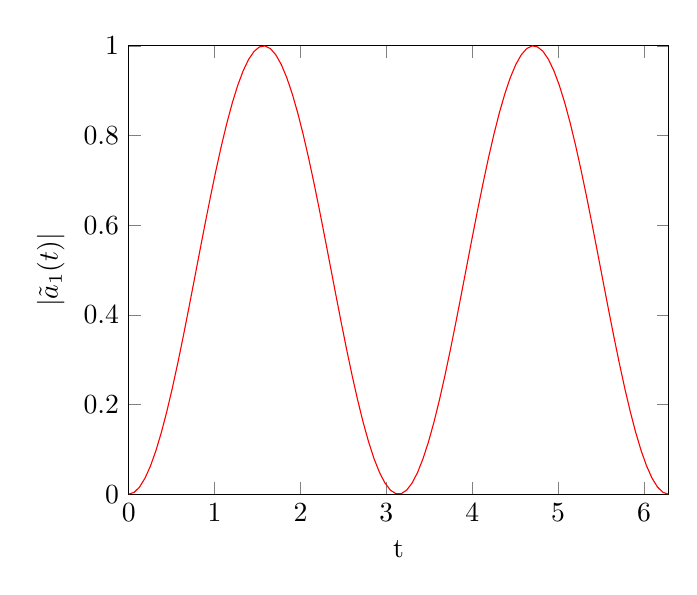
\begin{tikzpicture}
	\begin{axis}[
	    ylabel={$\left|\tilde{a}_1(t)\right|$},
	    xlabel=t,
	    xmin= 0, xmax= 2*pi,
	    ymin= 0, ymax =1,
	]
	\addplot[domain=0:2*pi, samples=100,color=red]{sin(deg(x))^2};
	\end{axis}
    \end{tikzpicture}
    \caption{$\left|\tilde{a}_1(t) \right|$ }
    \label{ddd}
\end{figure}
Il periodo di queste oscillazioni è $2\pi /\Omega_r$ , al tempo $\pi /\Omega_r = T_\pi$ il sistema si è "ribaltato": ha probabilità massima 1 di essere nel primo eccitato.
\begin{figure}[H]
    \centering
    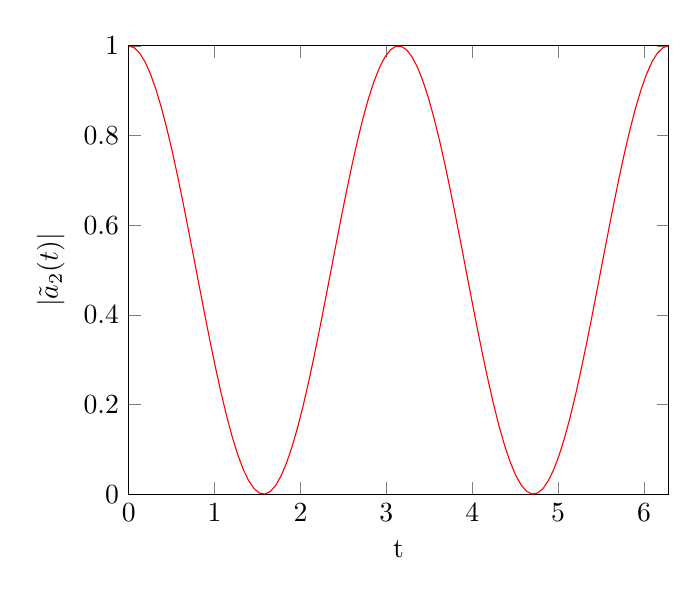
\begin{tikzpicture}
	\begin{axis}[
	    ylabel={$\left|\tilde{a}_2(t)\right|$},
	    xlabel=t,
	    xmin= 0, xmax= 2*pi,
	    ymin= 0, ymax =1,
	]
	\addplot[domain=0:2*pi, samples=100,color=red]{cos(deg(x))^2};
	\end{axis}
    \end{tikzpicture}
    \caption{$\left|\tilde{a}_2(t) \right|$.}
    \label{1111}
\end{figure}
Possiamo spiegarci questa cosa pensandola come tanti processi perturbativi consecutivi: il nostro atomo parte nel fondamentale ed interagendo con la radiazione passa nel primo eccitato. 
Arrivato nel livello eccitato non può più assorbire radiazione, può solo fare emissione stimolata ricadendo nel fondamentale.\\
Notiamo che la probabilità di transizione non è lineare nel tempo (come potevamo aspettarci per $\tau$ molto piccoli), inoltre tale soluzione deve contenere il trattamento perturbativo, quindi per tempi piccoli (ovvero tali da far rimanere la probabilità di transizione piccola). \\
Questo ci dice anche che l'approccio perturbativo vale per 
\[
\tau \ll \frac{2\pi}{\Omega_r}
.\] 
Possiamo anche risolvere le equazioni nel caso di $\delta \neq 0$, si ottiene:
\[
\left|\tilde{a}_1\right|^2= \frac{\Omega^2_r}{\Omega_r^2+\delta^2}
\sin^2\left(\frac{\sqrt{\Omega^2_r + \delta^2}}{2}t\right)
.\] 
Quindi la forma di $\left|\tilde{a}_1\right|^2$ si modifica nel seguente modo:
\begin{figure}[H]
    \centering
    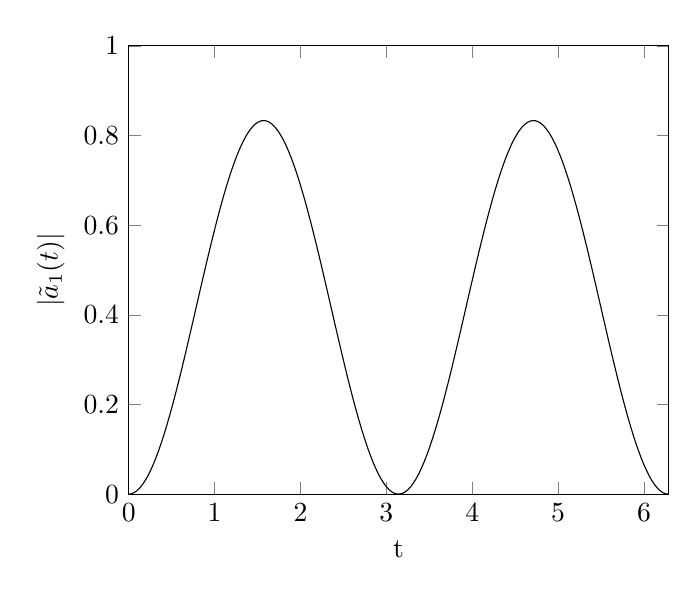
\begin{tikzpicture}
	\begin{axis}[
	    ylabel={$\left|\tilde{a}_1(t)\right|$},
	    xlabel=t,
	    xmin= 0, xmax= 2*pi,
	    ymin= 0, ymax = 1,
	]
	\addplot[domain=0:2*pi, samples=200]{5/6*sin(deg(x))^2};
	\end{axis}
    \end{tikzpicture}
    \caption{$\left|\tilde{a}_1(t)\right|$ considerando $\delta\neq 0$.}
    \label{delta non nullo}
\end{figure}
Con questa ultima equazione capiamo che l'approssimazione RWA è sensata, la correzione a questa sarebbero delle oscillazioni molto piccole sovrapposte all'andamento già oscillante. \\
Per poter visualizzare le onde di Rabi è necessario avere delle onde quanto più possibile monocromatiche, altrimenti la convoluzione di tutte le componenti oscillanti distruggerà la forma della oscillazione. \\
Per poter vedere tali oscillazioni quindi sarà necessario avere una ampiezza della distribuzione in frequenza $\Delta\omega$ pari a:
\[
\Delta\omega\ll\Omega_r
.\] 
Quindi gli esperimenti in questo campo si fanno tipicamente con Laser molto intensi.
\subsection{Interazione radiazione materia collegata alla termodinamica}%
\label{sub:Interazione radiazione materia collegata alla termodinamica}
Supponiamo di avere una Ensemble di N atomi, la probabilità al tempo $t$  di avere l'atomo nel livello $m$-esimo è $\left|a_m(t) \right|^2$. Il numero di atomi nel livello $m$-esimo al tempo $t$  sarà dato da:
\[
    N_m = N\left|a_m(t) \right|^2
.\] 
La probabilità di transizione l'abbiamo calcolata e supponiamo che gli atomi non abbiano altri tipi di interazione al di fuori del campo elettromagnetico. Possiamo quindi scrivere che:
\[
    \frac{\text{d} \left|a_n(t) \right|^2_\text{in} }{\text{d} t} =
    P_{m\to n}\left|a_m(t) \right|^2
.\] 
Viceversa:
\[
    \frac{\text{d} \left|a_m(t) \right|^2_\text{in} }{\text{d} t} =
    P_{n\to m}\left|a_n(t) \right|^2
.\] 
Questa è la probabilità che l'atomo vada nel livello $n$  per la prima formula e $m$  per la seconda.\\
La probabilità di uscire dal livello $n$  sarà invece:
\[
    \frac{\text{d} \left|a_n(t)\right|^2_\text{out} }{\text{d} t} =
    -\frac{\text{d} \left|a_n(t) \right|^2_\text{in} }{\text{d} t}=
    -P_{n\to m}\left|a_n\right|^2
.\] 
In totale (per tutti gli atomi) si ha che:
\[
\frac{\text{d} N_n}{\text{d} t} = \sum_{m}^{'} P_{m\to n}N_m 
-\sum_{m}^{'} P_{n\to m}N_n
.\] 
Le sommatoria sono su tutti i livelli diversi da $n$, la prima corrisponde al prodotto della probabilità di andare da $m$  a $n$  moltiplicata per gli atomi del livello $m$  (e poi sommiamo su tutti gli $m\neq n$) mentre il secondo termine corrisponde agli atomi che abbandonano il livello $n$.\\
Se siamo all'equilibrio ovviamente tale derivata deve essere nulla:
\[
\sum_{m}^{'} P_{m\to n}N_m =
\sum_{m}^{'} P_{n\to m}N_{n}
.\] 
Notiamo che stiamo ragionando sui moduli quadri delle ampiezze di probabilità, quindi quando facciamo una trattazione di rate abbiamo già perso un po di informazione (nella trattazione di Rabi invece potevamo vedere anche le fasi della ampiezza di probabilità), per questo motivo non siamo in grado di descrivere fenomeni coerenti o interferenze.\\
L'equazione per l'equilibrio che abbiamo trovato è parente di un'altra ancora più stringente che abbiamo già incontrato: l'equazione di bilancio dettagliato.\\
Infatti il bilancio dettagliato ci diceva che i singoli processi dai singoli stati devono essere uguali:
\[
\forall n,m \quad P_{m\to n}N_m = P_{n\to m}N_n 
.\] 
Dal punto di vista quantistico questa è strettamente connessa con il time revelsal simmetry.\\
Dal punto di vista classico (sistema alla Boltzmann) se prendiamo un sistema a due livelli sappiamo che all'equilibrio termico:
\[
    \frac{N_1^0}{N_2^0}= \frac{g_1}{g_2}\exp\left(-\frac{E_{12}}{kT}\right)
.\] 
Se gli atomi possono interagire solo con il campo elettromagnetico allora si ha che:
\[
P_{12} = B_{12}u_{\nu_{12}}=P_{21}=B_{21}u_{\nu_2}
.\] 
Applicando il bilancio dettagliato abbiamo che:
\[
\frac{N_1^0}{N_2^0} = \frac{P_{2\to 1}}{P_{1\to 2}} = 1
.\] 
Quindi sembra che le condizioni di equilibrio termodinamico e la condizione di equilibrio proveniente da un principio generale applicato all'interazione con il campo EM ci diano risultati diversi. \\
Einstein risolse questo problema assumendo che le probabilità fossero proporzionali alla intensità del campo elettromagnetico, egli introdusse un nuovo processo di emissione scrivendo:
\[
    P_{1\to 2}= B_{1\to 2}u_{\nu}(\nu_{12})  + A_{1\to 2}
.\] 
Il secondo termine è indipendente dalla densità di energia del campo elettromagnetico. Questo coefficiente è quello di emissione spontanea \footnote{Quantizzando il campo EM si vedrà che tale elemento viene fuori direttamente dagli elementi di matrice della interazione.}.\\
Possiamo ora scrivere le proprietà di equilibrio termodinamico:
\[
    \frac{N_1^0}{N_2^0} = \frac{B_{1\to 2 u_\nu(\nu_{12})}}{B_{1\to 2}u_\nu(\nu_{12}) + A_{1\to 2}} = \frac{g_1}{g_2}e^{-h\nu_{12} /k_BT}
.\] 
Possiamo quindi calcolare $A$  in funzione di $T$  :
\[
    A_{12} = \left(B_{1\to 2}\frac{g_2}{g_1}e^{h\nu_{12} /k_BT}-B_{1\to 2}\right)u_\nu(\nu_{12}) 
.\] 
Se siamo all'equilibrio termico possiamo utilizzare l'espressione di plank:
\[
A_{1\to 2} =
\frac{8\pi h\nu_{12}^3}{c^3}\left(\frac{B_{2\to 1}\frac{g_2}{g_1}e^{h\nu_{12} /k_BT}-B_{1\to 2}}{e^{h\nu_{12} /k_BT}-1}\right)
.\] 
Imponendo che tale coefficiente non dipenda dalla temperatura abbiamo che $B_{1\to 2}g_1=B_{2\to 1}g_2$, quindi rimane semplicemente:
\[
A_{1\to 2}=\frac{4}{3\hbar }\frac{\omega_{12}^3}{c ^3}\left|\bra{1}d\ket{2}\right|^2
.\] 
Questa è l'espressione del coefficiente di emissione spontanea, quella che si ottiene anche quantizzando il campo elettromagnetico.\\
Vediamo che dipende dal cubo della frequenza e dal modulo quadro del dipolo. Se siamo in una situazione di assenza del campo EM rimane l'emissione spontanea e troviamo dalla equazione di rate semplicemente un decadimento esponenziale con tempo caratteristico:
\[
\tau_{s}=\frac{1}{A_{1\to 2}}
.\] 
Diamo una dimensione numerica del tempo tipico di emissione spontanea:
\[
    \left|\bra{1}d\ket{2}\right|\approx ea \approx 2.4 \text{ Debye} = 2.4\cdot 10^{-30}\text{ [C][m]}
.\] 
Nel visibile ($\lambda\sim 600$ nm) abbiamo che il tempo di emissione spontanea viene $\tau_s \sim 100$  ns.\\
Se andiamo nell'infrarosso ($\lambda  = 10$ $\mu$m) abbiamo $\tau_s\sim 0.5$  ms.\\
Nel caso quantistico la trattazione fatta resta valida, tuttavia se cambiamo il tipo di particella sarà necessario cambiare l'assunzione che 
\[
\frac{\text{d} N_1}{\text{d} t} \propto N_{2}P_{21}
.\]   
Con particelle classiche questo funziona, con con particelle quantistiche invece no. \\
Prendiamo come esempio il caso di Fermioni: il rate con cui le particelle vanno dallo stato 1 a quello 2 deve tener conto del fatto che non ci può stare più di una particella per stato, gli stati finali devono essere liberi per transire.\\
Nel caso di Bosoni invece si ha che più particelle ci sono nello stato finale e più e probabile che un'altra particella ci finisca.\\
Vediamo adesso quando domina il processo di emissione stimolata e quando invece domina quello di emissione spontanea. Per far questo consideriamo il rapporto:
\[
    \frac{B_{1\to 2}u_\nu(\nu_{12})}{A_{1\to 2}} = \frac{1}{e^{h\nu_{12} /kT}-1}
    = n_\text{ph}^{(\nu_{12})} = n_{\nu_{12}}
.\] 
Questo è il numero medio di fotoni alla frequenza $\nu_{12}$  che è la frequenza della transizione. Quantizzando il campo magnetico troviamo che $P_\text{em} \propto n_\text{pH} + 1$, il primo termine sarà quello si emissione stimolata mentre quello di emissione spontanea è il secondo.\\
Questo comporta che in una situazione in cui $n_{\nu_{12}}\ll 1$ allora domina l'emissione spontanea, viceversa domina la stimolata.\\
Nel primo dei due casi se abbiamo fotoni termici la condizione comporta:
\[
e^{h\nu /kT}\ll 2
.\] 
Di conseguenza anche:
\[
    T\lambda\gg \frac{1}{\ln(2)}\frac{hc}{k}\sim 20000 [\mu\text{m}][\text{K}]
.\] 
L'emissione stimolata domina quindi per $\lambda\gg 10^4$.\\
\subsection{Applicazione dell'interazione radiazione materia: Laser}%
\label{sub:Applicazione dell'interazione radiazione materia: Laser}
Vediamo come varia l'intensità della radiazione quando attraversa un mezzo materiale (che noi schematizziamo come un sistema a due livelli). Dobbiamo studiare la variazione della intensità $I$  della radiazione (il flusso di energia per unità di tempo, la potenza per unità di area), ricordando che
\[
u = \frac{E_0^2}{8\pi}
.\] 
Questa è la densità di energia (nel corpo nero avevamo $u_\nu$: la densità di energia per unità di frequenza). Abbiamo quindi
\[
I=cu
.\] 
Considerando il seguente corpo
\begin{figure}[ht]
    \centering
    \incfig{corpo-per-interazione-radiazione-materia}
    \caption{Corpo per interazione radiazione materia}
    \label{fig:corpo-per-interazione-radiazione-materia}
\end{figure}
Vogliamo trovare l'andamento di $I_z$, in particolare vedremo che
\[
    I=\exp\left(-kz\right)I(0) 
.\] 
O in forma differenziale:
\[
    dI = -k I(z)dz
.\] 
Dove il segno negativo è per la convenzione che una variazione di intensità negativa si riferisce ad un $k$  positivo.\\
In generale $k$  potrebbe dipendere da $I$, al primo ordine non sarà così, $k$  si dice coefficiente di assorbimento.
Se tale parametro è positivo l'energia viene soppressa, se è negativo l'energia aumenta.\\
Per un sistema a due livelli questo significa che se $k$  è positivo l'energia viene persa dal campo elettromagnetico perché domina l'assorbimento, viceversa domina l'emissione stimolata.\\
Poniamoci nella situazione in cui $N_2$  ed $N_1$  (le popolazioni dei due livelli) sono fissate e diventano da qui in poi le densità di popolazione \footnote{Facciamo in modo che non si modifichino con l'applicazione di un campo elettromagnetico esterno}.
Consideriamo la variazione di $I$  in $z$  :
\[
\frac{\text{d} I}{\text{d} z} = c \frac{\text{d} u}{\text{d} z} 
= \frac{\text{d} z}{\text{d} t} \frac{\text{d} u}{\text{d} z} = \frac{\text{d} u}{\text{d} t} 
.\]
Ma l'ultima derivata la possiamo scrivere considerando che la densità di energia del campo EM cambia tramite processi di assorbimento o di emissione stimolata, trascuriamo l'emissione spontanea poiché consideriamo un campo elettromagnetico che si propaga con un vettore d'onda fissato nel nostro materiale. \\
Non abbiamo parlato le proprietà dei fotoni emessi nei vari processi, tuttavia i fotoni emessi per emissioni stimolata sono identici ai fotoni che li hanno stimolati, quelli emessi per emissione spontanea invece possono essere emessi in uno qualunque dei modi possibili del campo elettromagnetico, in particolare con un qualunque $k$. Per questo motivo li trascuriamo.\\
Abbiamo quindi processi di assorbimento o processi di emissione stimolata, per unità di tempo si produrranno tanti fotoni quanti atomi passano dal livello eccitato al fondamentale (per unità di tempo) e viceversa.
\[
\frac{\text{d} n^+}{\text{d} t} = \left|\frac{\text{d} N_1}{\text{d} t} \right|_\text{out} 
= P_{1\to 2}N_1
.\] 
\[
\frac{\text{d} n^-}{\text{d} t} =\left|\frac{\text{d} N_1}{\text{d} t} \right|_\text{out} = P_{2\to 1}N_2
.\] 
Quindi abbiamo che 
\[
\frac{\text{d} I}{\text{d} z} = \frac{\text{d} u}{\text{d} t} =
h\nu \left(P_{1\to 2}N_1 - P_{2\to 1}N_2\right)
.\] 
Inserendo dentro $P_{1\to 2}$  e $P_{2\to 1}$:
\[
    P_{1 \to 2} = B_{12}u_\nu (\nu_{12}) 
.\] 
Questa volta supponiamo che la radiazione sia molto "stretta" rispetto alla $g$, integriamo la $u_\nu$  lasciando la $g$.  \\
\[
    P_{1 \to 2} = B_{12}g(\nu-\nu_{12})u
.\] 
Inserendo dentro otteniamo l'espressione:
\[
    \frac{\text{d} I}{\text{d} z} = h\nu g(\nu-\nu_{12}) u\left(B_{1\to 2}N_1
    -B_{2\to 1}N_2\right)= -kI
.\] 
Nella formula abbiamo riscritto $u = I /c$  mentre il coefficiente $k$  vale:
\[
    k=\frac{h\nu}{c}g(\nu-\nu_{12})\left(B_{21}N_2 - B_{12}N_1\right) 
.\] 
All'equilibrio termodinamico la popolazione del livello i-esimo la popolazione sarà moltiplicata per la degenerazione del livello:
\[
N_i^0 = \frac{g_i e^{- E_i /kT}}{Z}
.\] 
Quindi abbiamo che:
\[
\frac{N_1^0}{N_2^0} = \frac{g_1}{g_2}e^{-E_{12} /kT}
.\] 
Inoltre
\[
\frac{B_{21}}{B_{12}} = \frac{g_1}{g_2}
.\] 
Anche con la degenerazione invece $A$ resta lo stesso. Supponiamo adesso che le degenerazioni siano uguali, il coefficiente di assorbimento diventa
\[
    k=\frac{h\nu}{c}g(\nu-\nu_{12}) (N_2-N_1) 
.\] 
Quindi il coefficiente di assorbimento è positivo quando $N_2$ è maggiore di $N_1$. \\
Se si riesce ad invertire la popolazione (cioè ad avere $N_1>N_2$) allora il coefficiente $k$ diventa negativo e la radiazione aumenta esponenzialmente nel passaggio nel materiale. 
